\chapter{函数的极限}
\label{chap:function-limits}
\label{chap:mathematical-analysis}

第~\ref{chap:sets-functions-and-proofs}章末尾的等比递推$e^{(t)}=\rho^te_0$给出了有限步结果；
当$t$无限增大时，这些数是否趋向确定的值？有限几何和在项数增加时又怎样变化？
本章先用数列的极限精确说明“趋近”，区分极限的计算与存在性判别；
再用部分和的极限研究级数的收敛，包括常见级数、收敛判别以及重排与保序分组的不同条件；
随后把极限从数列推广到函数。极限定义通过距离控制误差，最后在实轴上建立邻域、开闭集与闭区间的有限子覆盖性质，
这是一元函数微积分所需的部分；一般集合上的度量与紧致理论在随后的“度量空间”章展开。
这些认识为后续一元与多元微积分提供共同的极限语言。

\section{序列的极限}
\label{sec:analysis-continuous-limits}

数列$1,1/2,1/3,\ldots$越来越接近$0$，数列$-1,1,-1,1,\ldots$则在两个值之间来回交替。
直觉上前者“有极限”，后者没有；但“越来越接近”需要精确的含义，否则无法判断更复杂的情形，
例如$(1+1/n)^n$或$\sum_{k\leq n}1/k$是否趋向某个数。
极限用误差条件给出这种含义：给定任意小的误差，后面的项是否都能落在这一误差范围内。

\label{sec:analysis-sequences-series-errors}

有了定义以后，还要回答两类问题：已知几个数列收敛时，怎样计算由它们组合出的数列的极限；
尚不知道极限值时，怎样从数列本身的性质保证极限存在。前者借助极限的运算法则与夹逼，
后者依靠单调有界、收敛子列和柯西准则，这三种判别都要用到第~\ref{chap:sets-functions-and-proofs}章的确界原理。
本节先定义收敛并说明收敛数列有界，再建立存在性判别，然后讨论极限的唯一性、运算与夹逼，
最后用上、下极限描述不收敛数列尾部的上下边界。

\subsection{数列的收敛}

\paragraph{收敛与发散}
数列$(a_n)_{n\geq1}$是一列按正整数排列的实数。
“接近一个数”要同时约束后面的全部项，不能只看某几个位置：$((-1)^n)$的偶数项都等于$1$，
但奇数项始终离$1$有距离$2$，所以它不应算作趋于$1$。
只要求“各项与$a$的距离越来越小”也不够，例如$1+1/n$离$0$越来越近，却始终大于$1$。
合适的要求是：无论事先给定多小的正误差，从某一项起，后面\emph{每一项}与$a$的距离都小于这个误差。

若存在$a\in\mathbb R$，使每个$\varepsilon>0$都对应一个正整数$N$，满足
\[
 n\geq N\quad\Longrightarrow\quad |a_n-a|<\varepsilon,
\]
就称$(a_n)$\term{收敛}（converge）到$a$，$a$称为其极限，记作
$\lim_{n\to\infty}a_n=a$或$a_n\to a$。没有有限实数极限时，称数列发散（diverge）。
这里先任给误差$\varepsilon$，再选取$N$；选定以后，所有$n\geq N$都须满足要求。
$N$可以依赖于$\varepsilon$，误差要求越严格，所需的尾部起点通常越靠后；定义也不要求这个$N$唯一。
极限不要求某一项恰好等于$a$\scite{math-lebl-analysis1}。

例如对$a_n=1/n$，任给$\varepsilon>0$，取正整数$N>1/\varepsilon$，则$n\geq N$时
$|a_n-0|=1/n\leq1/N<\varepsilon$，所以$1/n\to0$。这样的整数$N$一定存在，因为正整数集合没有上界：
否则它有上确界$s$，而$s-1$不是上界，存在正整数$k>s-1$，于是正整数$k+1>s$，矛盾。

反过来，要说明$((-1)^n)$不收敛到任何$a$，只需取$\varepsilon=1$：
相邻两项相差$2$，不可能同时落在长度为$2$的开区间$(a-1,a+1)$内，所以没有$N$能使后面全部项满足要求。

图~\ref{fig:analysis-process-sequence-tail}把“全部尾部项”画成同一条误差带：选定起点以后，后面每一项都必须留在带内。
\begin{figure}[!htbp]
 \centering
 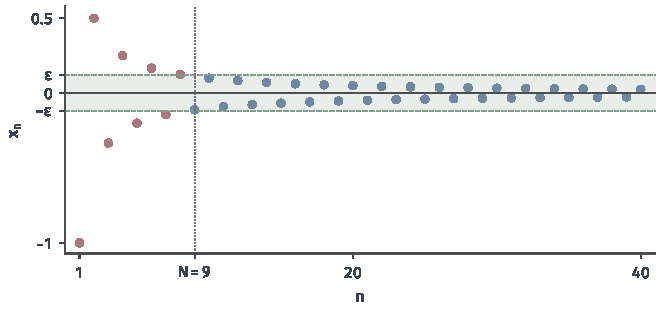
\includegraphics[width=112.0mm]{figures/01-mathematical-preliminaries-upper/00-shared/matplotlib/chapter3-concept-processes/sequence-tail.pdf}
 \caption{数列$x_n=(-1)^n/n$的前40项。绿色带为$|x_n|<0.12$，取$N=9$后，所有$n\geq9$都在带内；蓝点标记这个尾部，红点标记之前的项。尾部条件针对无限多个$n$，其成立依据是$1/n\leq1/9<0.12$，不是只检查图中有限个点。}
 \label{fig:analysis-process-sequence-tail}
\end{figure}

\paragraph{收敛数列的有界性}
收敛的定义只控制尾部，但尾部之前只有有限个项，因此收敛数列必有界。
设$a_n\to a$，取$\varepsilon=1$，得到$N$使$n\geq N$时$|a_n-a|<1$，从而$|a_n|<|a|+1$。
令$M=\max\{|a_1|,\ldots,|a_{N-1}|,|a|+1\}$，便有$|a_n|\leq M$对所有$n$成立。

反向结论不成立，例如$((-1)^n)$有界却不收敛：有界性只限制取值范围，没有控制尾部是否还在振荡。
这一性质常以逆否形式使用：无界数列一定发散。下一小节将看到，
有界性再配合单调性，或者只要求选出一部分项，就能得到收敛的结论。

\subsection{数列的收敛判别}

定义收敛时需要指定一个候选极限，但很多数列的候选极限尚不明确。
下面依次利用变化方向、取值范围和尾部各项的互相接近来判断极限是否存在，并说明各自需要的条件。

\subsubsection{单调数列的收敛}
若对所有$n$都有$a_n\leq a_{n+1}$，称数列单调不减；
若总有$a_n\geq a_{n+1}$，称数列单调不增，两者统称为单调数列。

对于单调不减且有上界的数列，第~\ref{sec:prelim-optimal-values-errors}节的确界原理
为全部项提供一个最小上界；单调性则保证后面的项一直靠近它。
\begin{theorem}[单调有界收敛定理]
\label{thm:analysis-monotone-bounded-sequence}
设$(a_n)_{n\geq1}$为实数列。
若$a_n\leq a_{n+1}$对所有$n\geq1$成立，且存在$M\in\mathbb R$使$a_n\leq M$对所有$n\geq1$成立，则
\[
 \lim_{n\to\infty}a_n=\sup\{a_n:n\geq1\}\in\mathbb R.
\]
若$a_n\geq a_{n+1}$对所有$n\geq1$成立，且存在$m\in\mathbb R$使$a_n\geq m$对所有$n\geq1$成立，则
\[
 \lim_{n\to\infty}a_n=\inf\{a_n:n\geq1\}\in\mathbb R.
\]
\end{theorem}
\begin{proof}
设$a=\sup\{a_n:n\geq1\}$。给定$\varepsilon>0$，$a-\varepsilon$不是上界，
所以存在$N$使$a_N>a-\varepsilon$。单调性使$n\geq N$时都有
$a-\varepsilon<a_N\leq a_n\leq a$，这正是$a_n\to a$。
单调不增的情形对$-a_n$应用同一论证。
\end{proof}
证明中只有一处用到实数的\term{完备性}（completeness）：非空上有界的实数集合$\{a_n:n\geq1\}$有实数上确界。
两个条件都不能省去：$(n)$单调却无上界，$((-1)^n)$有界却不单调。
结合收敛数列的有界性可知，单调数列收敛当且仅当它有界。

\subsubsection{有界数列的子序列收敛}
数列可能整体不收敛，但其中一些项仍有共同的趋向。保持原有次序选出一部分项，
得到子序列（subsequence），也称子列：若$n_1<n_2<\cdots$为严格递增的正整数列，
则$(a_{n_k})_{k\geq1}$为$(a_n)$的子序列。由归纳可知$n_k\geq k$。

收敛数列的每个子序列都收敛到同一极限：若$n\geq N$时$|a_n-a|<\varepsilon$，
则$k\geq N$时$n_k\geq k\geq N$，同一误差界仍然适用。
反过来，一个子序列收敛不能保证原数列收敛；$((-1)^n)$的偶数项恒为$1$，奇数项恒为$-1$。

有界数列未必收敛，但有界性能保证从中选出一个收敛子序列。
这一结论称为Bolzano--Weierstrass定理，随后将用它证明柯西条件足以保证实数列收敛。
\begin{theorem}[Bolzano--Weierstrass定理]
\label{thm:analysis-bounded-subsequence}
设$(a_n)_{n\geq1}$为实数列。若存在$M\geq0$使$|a_n|\leq M$对所有$n\geq1$成立，
则存在严格递增的正整数列$n_1<n_2<\cdots$和$a\in\mathbb R$，使
\[
 \forall\varepsilon>0,\quad\exists K\in\{1,2,\ldots\},\quad
 k\geq K\Longrightarrow |a_{n_k}-a|<\varepsilon.
\]
即$a_{n_k}\to a$。
\end{theorem}
\begin{proof}
从包含全部项的闭区间$I_0=[-M,M]$出发，将它平分，两半中至少有一半含有无穷多个下标对应的项；
选出这一半，再重复平分与选择，得到嵌套闭区间$I_0\supseteq I_1\supseteq\cdots$，
其中$I_k=[l_k,r_k]$含有无穷多项，长度为$2M\cdot2^{-k}$。
由$2^k\geq k+1$，这些长度至多为$2M/(k+1)$，因而趋于零；这里不必先用后面的等比数列极限。
由于每个$I_k$都含有无穷多项，可以依次选取下标$n_1<n_2<\cdots$，使$a_{n_k}\in I_k$。

再确定子序列的极限。各左端点$l_k$单调不减，而由嵌套性，每个$r_j$都是全部左端点的上界。
由确界原理，$c=\sup_k l_k$存在，并满足$l_k\leq c\leq r_k$对每个$k$成立。
给定$\varepsilon>0$，先选$K$使$r_K-l_K<\varepsilon$；
当$k\geq K$时，$a_{n_k}\in I_k\subseteq I_K$，且$c\in I_K$，所以$|a_{n_k}-c|\leq r_K-l_K<\varepsilon$。
\end{proof}

\subsubsection{柯西数列的收敛}
单调条件并不适用于所有收敛数列。若还不知道候选极限，可以检查尾部各项是否彼此接近。
满足
\[
 \forall\varepsilon>0,\quad\exists N,\quad
 \forall m,n\geq N,\quad |a_m-a_n|<\varepsilon
\]
的数列称为\term{柯西数列}（Cauchy sequence）。对实数列，这个条件与收敛等价。
\begin{theorem}[柯西收敛准则]
\label{thm:analysis-cauchy-convergence}
设$(a_n)_{n\geq1}$为实数列。存在$a\in\mathbb R$使$a_n\to a$，当且仅当
\[
 \forall\varepsilon>0,\quad\exists N\in\{1,2,\ldots\},\quad
 \forall m,n\geq N,\quad |a_m-a_n|<\varepsilon.
\]
\end{theorem}
\begin{proof}
每个收敛实数列都是柯西数列：若$n\geq N$时$|a_n-a|<\varepsilon/2$，则对$m,n\geq N$，
$|a_m-a_n|\leq|a_m-a|+|a_n-a|<\varepsilon$。

反过来，柯西条件先保证数列有界，论证与收敛数列的有界性相同，只是把极限换成尾部中的一项：
取误差$1$，所有$n\geq N$都满足$|a_n-a_N|<1$，前面有限个项另取最大绝对值即可。
由Bolzano--Weierstrass定理，可取子序列$a_{n_k}\to a$。

给定$\varepsilon>0$，选$N$使任意$m,n\geq N$满足$|a_m-a_n|<\varepsilon/2$，
再选一个$k$，使$n_k\geq N$且$|a_{n_k}-a|<\varepsilon/2$。
于是每个$n\geq N$都有
$|a_n-a|\leq|a_n-a_{n_k}|+|a_{n_k}-a|<\varepsilon$。
\end{proof}
这一准则的充分性通过收敛子列，仍然依赖实数的确界原理。

验证柯西条件时，可把两个较晚的项之间的距离估计为逐步变化的总和。对$m>n$，
\begin{equation}
 |a_m-a_n|\leq\sum_{k=n}^{m-1}|a_{k+1}-a_k|.
\label{eq:analysis-cauchy-tail-bound}
\end{equation}
仅有相邻差趋零还不够，因为中间的步数也在增加，必须控制整段和。
例如$a_1=0$、$a_{k+1}-a_k=1/k$时，每一步都趋零，但$a_{2n}-a_n=\sum_{k=n}^{2n-1}1/k$共有$n$项，
每项都大于$1/(2n)$，所以$a_{2n}-a_n>1/2$，它不是柯西数列，因而发散。
这里的$a_{n+1}$正是第~\ref{sec:analysis-series}节调和级数的前$n$项和：每一项都变小，累计却不稳定。

\subsection{极限的基本性质}

前面的判别给出了保证收敛的条件。现在假定实数列已经收敛，先说明极限唯一，
再分别计算和、差、数乘、积与商的极限，最后说明怎样用上下界夹逼求极限。
这些运算法则都以有限极限存在为前提，不能代替收敛性的判别。

\paragraph{极限的唯一性}
收敛数列的极限是唯一的。若$a\neq b$都是极限，
取$\varepsilon=|a-b|/3$，充分靠后的项应同时满足
$|a_n-a|<\varepsilon$和$|a_n-b|<\varepsilon$；
三角不等式却给出$|a-b|\leq|a-a_n|+|a_n-b|<2|a-b|/3$，矛盾。
因此记号$\lim_{n\to\infty}a_n$表示一个确定的数。

\paragraph{和的极限}
实际计算时，一个数列常由几个已知数列相加得到。设$a_n\to a$、$b_n\to b$，其中$a,b\in\mathbb R$，则
\[
 \lim_{n\to\infty}(a_n+b_n)=a+b.
\]
因为$|(a_n+b_n)-(a+b)|\leq|a_n-a|+|b_n-b|$，
只需让两个误差分别小于$\varepsilon/2$，便能使和的误差小于$\varepsilon$。

\paragraph{差的极限}
相减时也可以分别控制两列数的误差。在同样的有限收敛条件下，
\[
 \lim_{n\to\infty}(a_n-b_n)=a-b.
\]
这来自$|(a_n-b_n)-(a-b)|\leq|a_n-a|+|b_n-b|$，取尾部起点使右侧两项各小于$\varepsilon/2$即可。

\paragraph{数乘的极限}
把每一项乘以固定的实数$c$，只会把误差乘以$|c|$，所以
\[
 \lim_{n\to\infty}ca_n=ca.
\]
$c=0$时结论直接成立；$c\neq0$时，把原数列误差控制在$\varepsilon/|c|$以内即可。

\paragraph{积的极限}
乘积的误差还包含一个变化的因子，需要用到收敛数列的有界性。若$a_n\to a$、$b_n\to b$，则
\[
 \lim_{n\to\infty}a_nb_n=ab.
\]
取$M\geq1$使所有$|a_n|\leq M$，把误差拆成两部分：
\[
 |a_nb_n-ab|=|a_n(b_n-b)+b(a_n-a)|\leq M|b_n-b|+|b|\,|a_n-a|.
\]
让$|b_n-b|<\varepsilon/(2M)$、$|a_n-a|<\varepsilon/[2(|b|+1)]$同时成立，右侧便小于$\varepsilon$。

\paragraph{商的极限}
除法还须避免分母趋零。若$a_n\to a$、$b_n\to b$且$b\neq0$，则充分靠后的$b_n\neq0$，并且
\[
 \lim_{n\to\infty}\frac{a_n}{b_n}=\frac ab.
\]
事实上，取误差$|b|/2$，可知充分靠后的$|b_n|\geq|b|/2$，于是
$|1/b_n-1/b|=|b_n-b|/(|b_n||b|)\leq2|b_n-b|/|b|^2$，右侧趋于零；
前面有限个项不影响极限，再对$a_n\cdot(1/b_n)$用乘积规则即得结论。
例如将分子分母同除以$n$，得$n/(n+1)=1/(1+1/n)\to1$。
分母趋于零时不能套用此式：$0/0$与$\infty-\infty$一样，都不是可以直接计算的数值。

\paragraph{夹逼定理}
有时中间数列不断振荡，直接控制它的误差并不方便，但可以分别找到上下界。
若上下两列最终都靠近同一有限值，中间数列便被限制在同一误差范围内。
\begin{theorem}[夹逼定理]
\label{thm:analysis-sequence-squeeze}
设$(a_n)$、$(b_n)$、$(c_n)$为实数列。若存在正整数$N_0$使
\[
 \forall n\geq N_0,\qquad a_n\leq c_n\leq b_n,
\]
并且存在$\ell\in\mathbb R$满足
$\lim_{n\to\infty}a_n=\lim_{n\to\infty}b_n=\ell$，则
$\lim_{n\to\infty}c_n=\ell$。
\end{theorem}
\begin{proof}
任给$\varepsilon>0$，由两端收敛可选正整数$N_1,N_2$，使
$n\geq N_1$时$|a_n-\ell|<\varepsilon$，$n\geq N_2$时$|b_n-\ell|<\varepsilon$。
取$N=\max\{N_0,N_1,N_2\}$，则每个$n\geq N$都有
\[
 \ell-\varepsilon<a_n\leq c_n\leq b_n<\ell+\varepsilon.
\]
所以$|c_n-\ell|<\varepsilon$，按定义即$c_n\to\ell$。
\end{proof}
例如$-1/n\leq(\sin n)/n\leq1/n$，所以$(\sin n)/n\to0$。

一个反复使用的例子是$|r|<1$时$r^n\to0$。$r=0$时直接成立；
若$0<|r|<1$，写$1/|r|=1+h$，其中$h>0$。
先用归纳法证明$(1+h)^n\geq1+nh$：$n=1$时取等号；若它对$n$成立，则
$(1+h)^{n+1}\geq(1+nh)(1+h)=1+(n+1)h+nh^2\geq1+(n+1)h$。
因此$0<|r|^n\leq1/(1+nh)<(1/h)\cdot(1/n)\to0$，
再对$-|r|^n\leq r^n\leq|r|^n$用夹逼定理，得到$r^n\to0$。

这回答了章首关于等比递推~\eqref{eq:prelim-geometric-recurrence}的问题：
$|\rho|<1$时$e^{(t)}=\rho^te_0\to0$。另几种情形同样可以判断：设$e_0\neq0$，
$\rho=1$时各项恒为$e_0$；$\rho=-1$时各项在$\pm e_0$间交替，不收敛；
$|\rho|>1$时，同一不等式给出$|\rho|^t\geq1+th$（其中$|\rho|=1+h$），数列无界，因而发散。

\subsection{数列的上极限与下极限}
数列不收敛时，仍可考察其尾部的上下边界。
为记录无界的趋向，约定$a_n\to+\infty$表示对每个实数$M$，充分大的$n$都满足$a_n>M$；
$a_n\to-\infty$则要求最终都有$a_n<M$。
这两个符号不是有限实数极限，$\overline{\mathbb R}=\mathbb R\cup\{-\infty,+\infty\}$称为扩展实数，
其中$\infty-\infty$没有定义。

逐渐舍去前项时，尾部下界只会上升，尾部上界只会下降，因此可以分别用单调数列的极限记录它们。
\begin{definition}[数列的上极限与下极限]
\label{def:analysis-liminf-limsup}
对扩展实数列$(a_n)$，定义
\[
 \liminf_{n\to\infty}a_n
 =\lim_{n\to\infty}\inf_{k\geq n}a_k,
 \qquad
 \limsup_{n\to\infty}a_n
 =\lim_{n\to\infty}\sup_{k\geq n}a_k.
\]
右侧尾部下确界随$n$单调不减，尾部上确界随$n$单调不增，故两者的极限均在扩展实数中存在。
\end{definition}
这里的单调极限允许取$\pm\infty$：单调不减的数列有上界时由单调有界收敛定理收敛，
无上界时对每个$M$都有某一项超过$M$，此后各项也超过$M$，即趋于$+\infty$；单调不增的情形同理。

例如$((-1)^n)$的下极限为$-1$、上极限为$1$，通常极限不存在。
总有$\liminf a_n\leq\limsup a_n$，因为每个尾部的下确界不超过同一尾部的上确界。
二者同为有限值$a$当且仅当$a_n\to a$。若二者都等于$a$，则对给定$\varepsilon>0$，
充分靠后的尾部下确界大于$a-\varepsilon$、尾部上确界小于$a+\varepsilon$，夹在中间的每个尾部项都满足$|a_n-a|<\varepsilon$；
反之若$a_n\to a$，则$n\geq N$时尾部全落在$(a-\varepsilon,a+\varepsilon)$内，尾部的上下确界都在$[a-\varepsilon,a+\varepsilon]$中。
二者同为$+\infty$或$-\infty$时则对应上述无穷极限，仍应与有限实数收敛区别。

对有界实数列，上、下极限还可以由子序列达到。记$L=\limsup a_n$。
对每个$j$，先取足够晚的起点，使其后的尾部上确界小于$L+1/j$；
由于每个尾部的上确界都不小于$L$，这一尾部中又有某项大于$L-1/j$。
在下标超过前次所选下标的位置选出这样的项$a_{n_j}$，便有$|a_{n_j}-L|<1/j$，从而$a_{n_j}\to L$。下极限同理。

\FloatBarrier
\section{级数的收敛}
\label{sec:analysis-series}

有限和可以逐项相加，无限多项却无法“加完”。上一节的数列极限提供了处理办法：
把前$N$项的和看成一个数列，再问$N$无限增大时它是否趋向一个确定的数。
本节先用部分和定义级数及其收敛，再给出几何级数、裂项级数与$p$级数这些可作基准的例子；
随后分正项级数和变号级数建立收敛判别；最后说明改变求和次序与合并相邻项会怎样影响收敛和级数的和。

\subsection{级数的定义}
\label{sec:analysis-series-definition}

\paragraph{部分和}
给定数列$(a_n)_{n\geq1}$，把有限和的上限不断增大，就得到一个新的数列
\[
 s_N=\sum_{n=1}^{N}a_n=a_1+\cdots+a_N,
\]
$s_N$称为\term{部分和}（partial sum）。

\paragraph{无穷级数及其收敛}
符号\term{无穷级数}（infinite series）$\sum_{n=1}^{\infty}a_n$描述这一求和过程；
当$(s_N)$有有限极限$s$时，称级数收敛，并记$\sum_{n=1}^{\infty}a_n=s$；否则称级数发散。
例如$a_n=2^{-n}\to0$，而部分和$s_N=1-2^{-N}\to1$；
单项的极限与级数的和是两个不同的对象。

由$a_N=s_N-s_{N-1}$及差的极限法则可知，级数收敛必须有$a_N\to0$。反向则不成立：
上一节柯西数列部分的例子说明，调和级数$\sum_{n=1}^\infty1/n$的单项趋于零，部分和却不是柯西数列，因而发散。

级数是否收敛与前有限项无关：对任一固定的$m$，$\sum_{n=1}^\infty a_n$收敛当且仅当尾部$\sum_{n=m+1}^\infty a_n$收敛，
因为两者的部分和只相差固定的有限和$s_m$。此时$r_m=\sum_{n=m+1}^\infty a_n=s-s_m$称为余项，且$m\to\infty$时$r_m\to0$。

\paragraph{非负项级数的总和}
若所有$a_n\geq0$，部分和单调不减，因此有界时收敛，无界时趋于$+\infty$。
这种情形下统一记
\[
 \sum_{n=1}^{\infty}a_n:=\sup_N\sum_{n=1}^{N}a_n\in[0,+\infty].
\]
这是非负项级数的扩展总和；总和为$+\infty$时仍称级数发散，不把它混同于有限和。
这个记号对每个非负项级数都有意义，后面比较、重排和分组非负项时，都可以先在$[0,+\infty]$中比较总和，不必事先知道级数收敛。

\subsection{常见的级数}
\label{sec:analysis-common-series}

判断一般级数时，常把它与几类已经算清的级数比较。下面依次给出可以直接求和的几何级数与裂项级数，
以及收敛性由指数决定的$p$级数。

\paragraph{几何级数}
第~\ref{chap:sets-functions-and-proofs}章的有限几何和公式~\eqref{eq:prelim-finite-geometric-sum}给出$r\neq1$时
\[
 \sum_{n=0}^{N}r^n=\frac{1-r^{N+1}}{1-r}.
\]
当$|r|<1$时，前面的等比数列极限使$r^{N+1}\to0$，因而
\begin{equation}
 \sum_{n=0}^{\infty}r^n=\frac{1}{1-r}.
\label{eq:analysis-geometric-series}
\end{equation}
同一计算给出截断后的误差
$|\sum_{n=N+1}^{\infty}r^n|=|r|^{N+1}/|1-r|$。
若$|r|\geq1$，则$|r^n|\geq1$，单项不趋零，故级数发散。
几何级数既是一个可直接计算的例子，也提供比较其他级数尾部的基准。

\paragraph{裂项级数}
若每一项都能写成相邻两项之差$a_n=b_n-b_{n+1}$，第~\ref{chap:sets-functions-and-proofs}章的裂项求和公式~\eqref{eq:prelim-telescoping-sum}给出
$s_N=b_1-b_{N+1}$。因此级数收敛当且仅当$(b_n)$有有限极限$b$，此时$\sum_{n=1}^\infty a_n=b_1-b$。
例如$\frac1{n(n+1)}=\frac1n-\frac1{n+1}$，$b_n=1/n\to0$，故$\sum_{n=1}^\infty\frac1{n(n+1)}=1$。
裂项级数的部分和可以精确写出，因而与几何级数一样，可用作比较其他级数的基准。

\paragraph{$p$级数}
对于$\sum_{n=1}^{\infty}n^{-p}$，相邻项的比值趋于$1$，仅看单步下降不易区分不同的$p$。
可以将有限和按$n=2^k,\ldots,2^{k+1}-1$分成区块。
若$p>0$，每块有$2^k$项，块内每一项都介于$(2^{k+1})^{-p}$与$(2^k)^{-p}$之间，乘以项数得
\[
 2^{-p}2^{k(1-p)}
 \leq\sum_{n=2^k}^{2^{k+1}-1}n^{-p}
 \leq2^{k(1-p)}.
\]
任一部分和$s_N$都不超过前$K+1$个整块之和$s_{2^{K+1}-1}$，其中$2^{K+1}-1\geq N$，所以对整块的估计控制了全部部分和。
这里只比较有限区块，尚未调用无穷级数的分组规则。

$p>1$时，右侧随$k$构成公比$2^{1-p}<1$的几何级数，于是每个部分和都不超过$1/(1-2^{1-p})$；
由非负部分和的单调性，级数收敛。$0<p\leq1$时，$2^{k(1-p)}\geq1$，每块至少为$2^{-p}$，累计任意多块便无界。
$p\leq0$时原级数的单项已不趋零。因此$p$级数恰在$p>1$时收敛；
特别地，调和级数$\sum_{n=1}^{\infty}1/n$发散。

\subsection{级数的收敛判别}
\label{sec:analysis-series-tests}

判断级数收敛，就是判断部分和是否有有限极限。非负项的部分和单调，可以用上界控制；
出现正负项后，还须区分绝对值累计有限与依靠抵消才收敛的两种情形。

\subsubsection{正项级数}

\paragraph{比较判别法}
几何级数与$p$级数已提供两个基准。对一般正项级数，可以先比较单项，
再用非负部分和的单调性把大小关系传递到总和。
若充分大的$n$都有$0\leq a_n\leq b_n$，则
$\sum b_n$收敛蕴含$\sum a_n$收敛；$\sum a_n$发散蕴含$\sum b_n$发散。
这称为比较判别法，有限个前项不影响收敛。
例如$n\geq1$时$1/[n(n+1)]\leq1/n^2$，由$p=2$的情形也可知前者的级数收敛。

单项比值趋于正常数时，也可以直接比较。
若$a_n,b_n>0$且$a_n/b_n\to c\in(0,\infty)$，则最终
$(c/2)b_n\leq a_n\leq(3c/2)b_n$，两级数因而同收敛或同发散，称为极限比较判别法。

\paragraph{比值判别法}
另一种比较从相邻项的比例入手。设$a_n>0$且$a_{n+1}/a_n\to r$。
当$r<1$时，可选$r<q<1$，使充分靠后都有$a_{n+1}\leq qa_n$，
逐次代入得到$a_{N+j}\leq a_Nq^j$，用几何级数比较便知收敛。
当$r>1$时，充分靠后的项递增而不趋零，级数发散；比值趋于$+\infty$亦同。
这称为比值判别法。

$r=1$时无法据此判断：收敛的$\sum1/n^2$与发散的$\sum1/n$
都有相邻项比值趋于$1$，必须另用比较等方法。

\subsubsection{变号级数}

\paragraph{绝对收敛与条件收敛}
项的正负交替或不规则变化时，部分和失去单调性，正负抵消也会影响累计。
若实数级数$\sum a_n$的绝对值级数$\sum|a_n|$收敛，称原级数
\term{绝对收敛}（absolute convergence）；若原级数收敛但$\sum|a_n|$发散，则称为条件收敛（conditional convergence）。
绝对收敛意味着即使不依赖抵消，累计的绝对贡献仍有限。
条件收敛则要求同时证明原级数收敛和绝对值级数发散；只知道后者，不能排除原级数也发散。

\paragraph{绝对收敛的判定}
判断绝对收敛只需对非负项级数$\sum|a_n|$使用比较或比值判别；若它收敛，原级数便必收敛。
理由是对$m>n$有
\[
 |s_m-s_n|\leq\sum_{k=n+1}^{m}|a_k|\leq\sum_{k>n}|a_k|,
\]
右侧是收敛非负级数的余项，与$m$无关且随$n$增大趋于零，故$(s_n)$满足柯西准则。
因此绝对收敛蕴含收敛，判断时不必先单独证明原级数收敛。
例如$\sum(-1)^{n+1}/n^2$由$p=2$的情形得到绝对收敛。

若级数和为$s$，在上式中令$m\to\infty$（若极限大于右侧的固定数，充分靠后的$|s_m-s_n|$也会大于它），得到
\[
 |s-s_N|\leq\sum_{n>N}|a_n|\longrightarrow0,
\]
即绝对尾和是截断误差的上界。

\paragraph{条件收敛的判定}
绝对值级数发散后，还须判断原级数中的抵消是否足以使部分和稳定。
最基本的条件是：$b_n\geq0$单调不增且$b_n\to0$时，
交错级数$\sum_{n=1}^{\infty}(-1)^{n+1}b_n$收敛，这称为Leibniz判别法。

其偶数部分和单调不减，奇数部分和单调不增，且每个偶数部分和都不超过任何奇数部分和。
因此偶数部分和以$s_1$为上界，奇数部分和以$s_2$为下界，两列分别收敛；
相邻的奇偶部分和之差$s_{2n+1}-s_{2n}=b_{2n+1}\to0$，两个极限因而相同。
给定误差后，奇偶两类下标的尾部分别满足要求，取较晚的起点即知原部分和收敛。
级数和位于任意一对相邻的奇偶部分和之间，因此余项绝对值不超过$b_{N+1}$。

例如$\sum(-1)^{n+1}/n$收敛，绝对值级数却是调和级数，所以条件收敛。
若$\sum b_n$本来就收敛，Leibniz条件给出的交错级数则是绝对收敛，不能一概称为条件收敛。

更一般地，若$A_N=\sum_{n=1}^{N}a_n$一致有界，即存在$M$使$|A_N|\leq M$对所有$N$成立，
而$b_n\geq0$单调趋零，则$\sum a_nb_n$收敛，这称为Dirichlet判别法。
这里$a_n$提供有界振荡，$b_n$使振荡的权重趋零。

为说明二者如何配合，对$m\leq k$记$A_k^{(m)}=\sum_{n=m}^{k}a_n=A_k-A_{m-1}$，则$|A_k^{(m)}|\leq2M$。
把$a_k=A_k^{(m)}-A_{k-1}^{(m)}$代入有限和并整理，得到
\[
 \sum_{k=m}^{N}a_kb_k
 =A_N^{(m)}b_N+
   \sum_{k=m}^{N-1}A_k^{(m)}(b_k-b_{k+1}),
 \qquad A_{m-1}^{(m)}=0.
\]
由于$b_k-b_{k+1}\geq0$，这段和的绝对值不超过
$2M[b_N+\sum_{k=m}^{N-1}(b_k-b_{k+1})]=2Mb_m$，它与$N$无关且随$m$增大趋于零，由柯西准则得证。

取$a_n=(-1)^{n+1}$便回到交错情形。
该判别只保证原级数收敛；是否条件收敛，还须另外证明$\sum|a_nb_n|$发散。

图~\ref{fig:analysis-process-series-terms-sums}并排比较级数的项与部分和。两列项都趋零，累计后的行为仍然不同。
\begin{figure*}[!htbp]
 \centering
 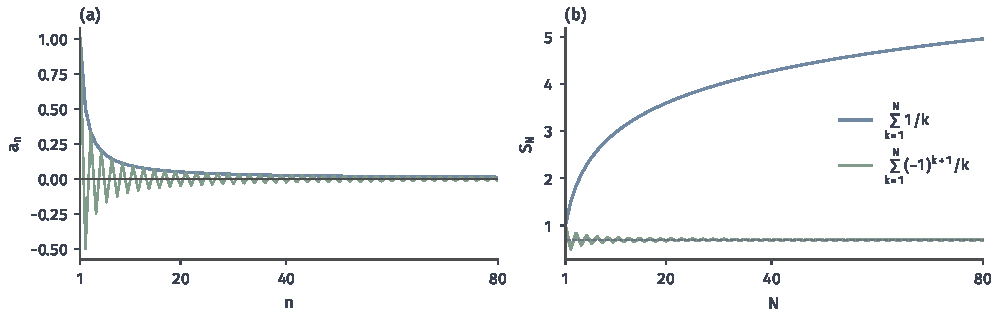
\includegraphics[width=169.0mm]{figures/01-mathematical-preliminaries-upper/00-shared/matplotlib/chapter3-concept-processes/series-terms-sums.pdf}
 \caption{(a) 蓝、绿折线分别连接$1/n$与$(-1)^{n+1}/n$的前80项。(b) 对应的部分和：调和部分和继续增长，交错调和部分和趋于虚线所示的$\log2$。项趋零只是级数收敛的必要条件；图展示有限段，收敛或发散由前面的判别证明。}
 \label{fig:analysis-process-series-terms-sums}
\end{figure*}

\subsection{级数的重排和分组对收敛的影响}
\label{sec:analysis-series-rearrangement-grouping}

收敛判别处理的是原次序下的部分和。接下来改变求和的组织方式：重排改变各项的次序，
分组只把原次序中的有限个相邻项合并；两种操作对收敛性的影响不同，需要分别检验。

\paragraph{级数的重排}
有限和可以交换项的先后；无穷级数则要检查新的部分和如何覆盖旧项。
若$\pi:\{1,2,\ldots\}\to\{1,2,\ldots\}$为双射，$\sum_{n=1}^{\infty}a_{\pi(n)}$称为原级数的重排，
它每项恰好使用一次，改变的是各项进入累计的顺序。

对于非负项，重排的每个部分和只含有限个原下标，这些下标都不超过某个$N$，所以它不超过$s_N$，从而不超过原扩展总和；
反过来，原来的任意前$N$项也会全部进入重排的某个有限前段。对两个方向分别取上确界，便知重排保持总和，允许总和为$+\infty$。

绝对收敛也保证任意重排保持原和。设原级数和为$s$，记重排的部分和为$t_K=\sum_{n=1}^{K}a_{\pi(n)}$。
给定$\varepsilon>0$，先选$N$使$\sum_{n>N}|a_n|<\varepsilon$，再选$K_0$使$\pi(1),\ldots,\pi(K_0)$已包含$1,\ldots,N$。
当$K\geq K_0$时，$t_K-s_N$是若干个下标大于$N$的项之和，故$|t_K-s_N|\leq\sum_{n>N}|a_n|<\varepsilon$；
又由前面的截断误差界，$|s_N-s|<\varepsilon$。因此$|t_K-s|<2\varepsilon$，重排仍收敛到$s$。

条件收敛没有这一保证。记$P_N$、$Q_N$分别为前$N$项中正项之和与负项绝对值之和，
$P$、$Q$为相应的扩展总和。若其中一个有限，由$s_N=P_N-Q_N$收敛会推出另一个也有限，
于是$\sum|a_n|=P+Q$有限，与条件收敛矛盾，故二者都为$+\infty$。

对任意实数目标$L$，可以按原先的相对次序取正项，直到部分和超过$L$，
再取负项直到低于$L$，如此反复；每次都至少取一项相应符号的项。
由于$P=Q=+\infty$，每一轮都会在有限步内结束，两类项最终都被用到；
而$a_n\to0$使每次越过$L$的幅度趋零，因此得到和为$L$的重排。
原级数若含零项，每轮再按原次序插入下一个尚未使用的零项（若有）；这不改变和，并保证每个零项也最终被用到。
也可交替超过$1$、低于$0$，构造不收敛的重排。
可见条件收敛级数的和依赖抵消的顺序，不能按有限和的交换律任意调换。

\paragraph{级数的分组}
分组保持原项的顺序，只将有限个相邻项合为一项。
准确地说，取$0=n_0<n_1<n_2<\cdots$，令
$b_j=\sum_{k=n_{j-1}+1}^{n_j}a_k$，则分组后前$J$项的和恰为$s_{n_J}$。
所以原级数收敛到$s$时，分组后的部分和是原部分和的子序列，也必收敛到$s$；
这对绝对收敛和条件收敛都成立。

反向不成立。级数$1-1+1-1+\cdots$的部分和在$1$与$0$之间交替，原级数不收敛，
但按$(1-1)+(1-1)+\cdots$分组后各项为零。
分组只保留部分截断位置，可能掩盖块内的振荡。

非负项没有这种抵消：原部分和单调，分组截断又越过每一个原截断位置，
两者的上确界相同，故即使总和为$+\infty$也可保序分组。
结合非负项的重排规则，可先把非负项按任意编号排列，再分成有限相邻块，而不改变扩展总和；
后面构造外测度时，将用这些求和性质累计覆盖区间的长度。

\FloatBarrier
\section{函数的极限}
\label{sec:analysis-function-limits}

数列的指标按自然数逐项增加，函数的输入却可以从许多实数位置靠近同一点。例如$(x^2-1)/(x-1)$在$x=1$没有定义，但在$x\neq1$时它等于$x+1$，所以邻近输入的输出仍趋于$2$。函数极限研究的正是这种去掉中心点后的共同趋近，不要求函数在中心有取值。

\subsection{函数极限的定义}
\paragraph{聚点}

讨论输入接近$a$之前，须保证定义域中确实有不同于$a$的输入能够任意靠近$a$。
设$X\subseteq\mathbb R$。若每个$r>0$都能找到$x\in X$使$0<|x-a|<r$，
即$(a-r,a+r)$去掉$a$以后（称为$a$的去心邻域）总含有$X$中的点，就称$a$为$X$的\term{聚点}（cluster point）。
例如$0$是$(0,1)$的聚点，虽然$0$不属于这个集合。
$X$中不是聚点的点称为$X$的\term{孤立点}（isolated point），例如整数集合中的每个点；
在孤立点附近没有其他输入，谈不上“趋近”。

\paragraph{函数极限}
有了能够趋近的输入，还要用输入误差控制输出误差，这与数列极限比较尾部误差的思路相同。
设$f:X\to\mathbb R$，$a$为$X$的聚点，$b\in\mathbb R$。
若对每个$\varepsilon>0$，都存在$\delta>0$使
\[
 x\in X,\quad0<|x-a|<\delta\quad\Longrightarrow\quad|f(x)-b|<\varepsilon,
\]
就称$b$为$x\to a$时$f(x)$的极限，记作$\lim_{x\to a}f(x)=b$。
也就是说，只要输入与$a$足够近，输出与$b$的距离就能任意小。

定义中的$0<|x-a|$排除了中心点，所以既不要求$f(a)$有定义，也不要求它等于$b$。
回到开头的例子$f(x)=(x^2-1)/(x-1)$：对$x\neq1$有$f(x)=x+1$。
给定$\varepsilon>0$，取$\delta=\varepsilon$，则
$0<|x-1|<\delta$时$|f(x)-2|=|x-1|<\varepsilon$，所以其极限为$2$。

图~\ref{fig:analysis-process-epsilon-delta-band}将输入邻域与输出误差带对应起来，同时把基点取值与趋近时的极限分开。
\begin{figure}[!htbp]
 \centering
 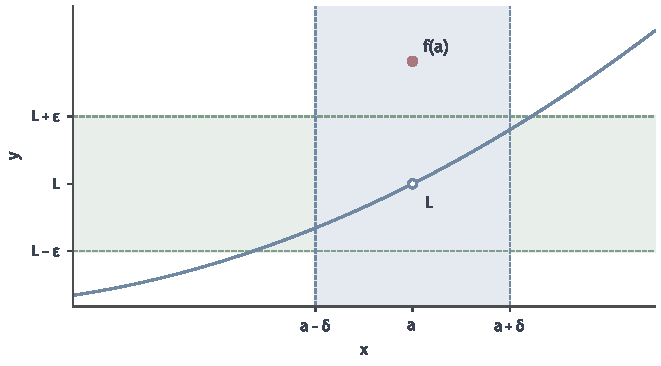
\includegraphics[width=112.0mm]{figures/01-mathematical-preliminaries-upper/00-shared/matplotlib/chapter3-concept-processes/epsilon-delta-band.pdf}
 \caption{取$a=L=1$（$L$即正文中的极限值$b$），$x\neq1$时$f(x)=x^2$，另令$f(1)=2$。蓝带对应$\delta=0.2$的输入范围，绿带对应$\varepsilon=0.55$的输出范围；去掉$a$后，蓝带内曲线全部落在绿带内。空心点是极限位置，红实心点是$f(a)$，不参加去心邻域条件。}
 \label{fig:analysis-process-epsilon-delta-band}
\end{figure}

\paragraph{左极限与右极限}
实轴上的输入可以从一个点的两侧接近，而两侧的输出未必有相同趋向，因此先分别考察每一侧的极限。
只让$x<a$的点趋近$a$，得到左极限$\lim_{x\uparrow a}f(x)$；
只让$x>a$的点趋近$a$，得到右极限$\lim_{x\downarrow a}f(x)$。
两种定义分别在上述误差条件中增加$x<a$或$x>a$，
并要求相应一侧存在定义域中的点任意靠近$a$。
若两侧都能趋近$a$，双侧极限存在当且仅当左右极限都存在且相等。

例如$f(x)=\mathbb I\{x\geq0\}$在$0$处的左右极限分别为$0$和$1$，所以双侧极限不存在。
这里$\mathbb I$为指示函数：括号内条件成立时取$1$，否则取$0$。
在定义域$[a,b]$内，只能从右侧趋近左端点$a$，从左侧趋近右端点$b$。
这种左右判据依赖实轴上的顺序，多元函数还须控制其他趋近方式。

\paragraph{无穷远处的极限}
输入也可以趋于无穷。设定义域向右无界，条件
\[
 \lim_{x\to+\infty}f(x)=b
\]
表示：对每个$\varepsilon>0$，存在$M$，使定义域中所有$x>M$都满足$|f(x)-b|<\varepsilon$。
定义域向左无界时，$x\to-\infty$的定义相应要求所有$x<M$的允许输入满足同一误差界。
例如$1/x$在$x\to+\infty$和$x\to-\infty$时都趋于$0$。

\paragraph{值为无穷的极限}
前一段改变的是输入的趋向；即使输入趋近有限点，输出也可能越过任何有限界，因此还需要描述输出本身的无界趋向。
对有限聚点$a$，$f(x)\to+\infty$（$x\to a$）是指：对每个实数$M$，都存在$\delta>0$，使定义域中满足$0<|x-a|<\delta$的每个$x$都有$f(x)>M$。
趋于$-\infty$则把最后的不等式改为$f(x)<M$。单侧无穷极限再限制输入所在的一侧。
因此$1/x$在$x\downarrow0$时趋于$+\infty$，在$x\uparrow0$时趋于$-\infty$，并没有共同的双侧无穷极限。

\subsection{常见函数的极限}

\paragraph{三角函数}
三角函数的自变量采用弧度制：单位圆上弧长为$h$的圆心角记为$h$。
比较内接三角形、扇形和外切三角形的面积，可得$0<h<\pi/2$时
$\sin h\leq h\leq\tan h$，从而$\cos h\leq\sin h/h\leq1$。
又由$1-\cos h=2\sin^2(h/2)\leq h^2/2$得到误差界
\[
 0\leq1-\frac{\sin h}{h}\leq1-\cos h\leq\frac{h^2}{2}.
\]

任给$\varepsilon>0$，只要$0<h<\min\{\pi/2,\sqrt{2\varepsilon}\}$，第一个比值与$1$的误差就小于$\varepsilon$；
$\sin h/h$是偶函数，所以同一估计也控制$h<0$的一侧。
第二个比值由$|1-\cos h|/|h|\leq|h|/2$控制，这个误差界对正负两侧都适用。因此
\[
 \lim_{h\to0}\frac{\sin h}{h}=1,
 \qquad
 \lim_{h\to0}\frac{\cos h-1}{h}=0.
\]
弧度制使第一个极限恰为$1$，用角度制时会多出比例系数。

\paragraph{自然指数函数}
后面求指数函数的导数需要一个原点处的基本极限。下面先用级数构造自然指数函数并验证其收敛，
再建立乘法性质和局部变化关系。定义
\[
 \exp x=\sum_{k=0}^{\infty}\frac{x^k}{k!}.
\]
对固定$x$，相邻项绝对值之比为$|x|/(k+1)$，当$k+1\geq2|x|$时不超过$1/2$，
尾部被几何级数控制，所以级数绝对收敛。

为得到乘法性质，先考察两个绝对收敛级数$\sum_k a_k$与$\sum_j b_j$的乘积。有限的正方形和满足
$\sum_{k=0}^N\sum_{j=0}^Na_kb_j=(\sum_{k=0}^Na_k)(\sum_{j=0}^Nb_j)$，
所以它们趋于两级数和的乘积。按总次数$k+j=n$合并的三角形部分和$\sum_{n=0}^{N}\sum_{k+j=n}a_kb_j$，
与正方形和只差满足$k,j\leq N$、$k+j>N$的项；这些项的$k$或$j$大于$N/2$，其绝对值之和不超过
$(\sum_{k>N/2}|a_k|)(\sum_j|b_j|)+(\sum_k|a_k|)(\sum_{j>N/2}|b_j|)$，它随$N$增大趋于零。
因此按总次数合并后也得到同一极限。

把这个结论用于指数级数，记
$C_n=\sum_{k=0}^n x^ky^{n-k}/[k!(n-k)!]$。将系数$n$拆为$k+(n-k)$，并分别换一次有限求和的索引，得到
\[
 nC_n=(x+y)C_{n-1},\qquad n\geq1.
\]
由$C_0=1$逐步得到$C_n=(x+y)^n/n!$，因而
\[
 \exp x\,\exp y
 =\sum_{n=0}^{\infty}\sum_{k=0}^n\frac{x^ky^{n-k}}{k!(n-k)!}
 =\sum_{n=0}^{\infty}\frac{(x+y)^n}{n!}
 =\exp(x+y).
\]
记$e=\exp1$，$e$约为$2.71828$。由加法公式，对正整数$n$有$\exp n=e^n$，
因此通常把$\exp x$写作$e^x$，称为以$e$为底的指数函数。

当$0<|h|<1/2$时，利用$1/k!\leq1$直接估计级数的二阶以后各项：
\[
 |e^h-1-h|
 \leq\sum_{k=2}^{\infty}|h|^k
 =\frac{h^2}{1-|h|}\leq2h^2.
\]
除以$|h|$得$|(e^h-1)/h-1|\leq2|h|$，令$h\to0$，就有
\[
 \lim_{h\to0}\frac{e^h-1}{h}=1.
\]
这一推导只用到级数，未使用求导或积分。

加法公式还给出其他性质。由$e^xe^{-x}=e^0=1$知$e^x\neq0$，又$e^x=(e^{x/2})^2\geq0$，因此$e^x>0$。
对$u\geq0$，级数各项非负，只保留前两项便得
\[
 e^u\geq1+u\qquad(u\geq0),
\]
这一不等式给出指数函数在非负半轴上的一个线性下界。
对$h>0$，由此$e^h\geq1+h>1$，于是$e^{x+h}=e^xe^h>e^x$，指数函数严格递增。
同一估计说明$x\to+\infty$时$e^x\to+\infty$；由$e^x=1/e^{-x}$又得$x\to-\infty$时$e^x\to0$。
对固定$x$和$|h|<1/2$，上述余项界还给出$|e^{x+h}-e^x|=e^x|e^h-1|\leq e^x(|h|+2h^2)\to0$。
这些性质将在连续函数的介值定理建立后，用于构造自然对数这一反函数
\scite{math-lebl-analysis1}。

\subsection{函数极限的性质与运算}
\paragraph{序列判据}

函数极限要求控制$a$附近所有允许的输入。这个条件等价于：每列满足$x_n\in X\setminus\{a\}$且$x_n\to a$的输入，都有$f(x_n)\to b$。

正向，给定$\varepsilon$后取函数极限中的$\delta$，充分靠后的$x_n$满足$0<|x_n-a|<\delta$，于是$|f(x_n)-b|<\varepsilon$。
反向用反证法。若误差条件不成立，就存在$\varepsilon_0>0$，使每个$1/n$去心邻域内都能选到$x_n\in X$，满足$|f(x_n)-b|\geq\varepsilon_0$；
这列输入趋于$a$，输出却不趋于$b$，与序列条件矛盾。

\paragraph{和的极限}
序列判据把函数极限转化为数列极限，从而可以逐项借用数列极限的运算法则。
以下各段统一设$f,g:D\to\mathbb R$，$a$为$D$的聚点，且在$x\in D$、$x\to a$时
$f(x)\to b$、$g(x)\to c$，其中$b,c\in\mathbb R$。和的极限为
\[
 \lim_{x\to a}(f(x)+g(x))=b+c.
\]
任取$x_n\in D\setminus\{a\}$且$x_n\to a$，序列判据给出$f(x_n)\to b$、$g(x_n)\to c$；
数列和的法则给出$f(x_n)+g(x_n)\to b+c$。由于对任意这样的输入列都成立，再用序列判据即得结论。

\paragraph{差的极限}
相减也保留有限极限关系：
\[
 \lim_{x\to a}(f(x)-g(x))=b-c.
\]
对每列趋于$a$的允许输入，数列差的法则都给出相应输出差趋于$b-c$，再由序列判据返回函数极限。

\paragraph{数乘的极限}
固定倍数只按比例改变输出误差。对任意固定$\lambda\in\mathbb R$，
\[
 \lim_{x\to a}\lambda f(x)=\lambda b.
\]
沿任意允许输入列使用数列常数倍的极限，再用序列判据即可；$\lambda=0$时输出恒为零。

\paragraph{积的极限}
两个有限极限也可以分别相乘：
\[
 \lim_{x\to a}f(x)g(x)=bc.
\]
沿任意允许输入列应用数列乘积的法则，得到输出积趋于$bc$；序列判据保证这控制了$a$附近的全部允许输入。

\paragraph{商的极限}
商需要额外要求分母极限$c\neq0$，此时
\[
 \lim_{x\to a}\frac{f(x)}{g(x)}=\frac bc.
\]
先取输出误差$|c|/2$，便知$a$的某个去心邻域内有$|g(x)|>|c|/2>0$，商在那里有定义。
在这一邻域内，任意输入列都可使用数列的商法则，再由序列判据得到结论。

若分子分母都趋于零，就不能套用此式。例如$(x^2-1)/(x-1)$在$x\to1$时须先约去公因子$x-1$，才能求出极限$2$。
同样，$\infty-\infty$等形式也须先变形或另外估计。

\paragraph{夹逼定理}
不易直接分解的函数，可以用同趋向的两侧函数控制。设在$a$的某个去心邻域内，所有允许输入满足
$u(x)\leq h(x)\leq v(x)$，且$u(x)\to L$、$v(x)\to L$，其中$L\in\mathbb R$，则
\[
 \lim_{x\to a}h(x)=L.
\]
任给$\varepsilon>0$，取一个共同的去心邻域，使其中$u(x)$和$v(x)$都落在$(L-\varepsilon,L+\varepsilon)$内，
夹在中间的$h(x)$也在其中。例如$-|x|\leq x\sin(1/x)\leq|x|$在$x\neq0$时成立，因此$x\to0$时$x\sin(1/x)\to0$。

\subsection{无穷小与无穷大}

\paragraph{无穷小}
趋向零的量可以出现在数列、函数或后面的微分余项中，先给这类趋向一个统一名称。
在指定的趋向下，极限为$0$的函数（或数列）称为无穷小（infinitesimal）。
例如$x\to0$时，$x$和$x^2$都是无穷小；$n\to\infty$时，$1/n$也是无穷小。
“无穷小”描述变化过程中的极限性质，不是某个固定的很小的非零数。

\paragraph{无穷大}
函数值的绝对值也可能最终超过任意固定门槛，这种趋向与趋零可以通过倒数联系起来。
在指定的趋向下，若$|f(x)|\to+\infty$，则称$f$为无穷大。
例如$x\to0$时，$1/x$为无穷大，但它没有共同的正或负无穷极限。
若$f$在所考察的趋向附近非零，则$|f|\to+\infty$等价于$1/f\to0$。

\paragraph{渐近记号}
\label{sec:comb-growth-scales}
两个函数即使同为无穷小，趋零的相对速度也可以不同。
设在所讨论的趋向附近$g\neq0$，定义
\[
 f=o(g)\quad\text{表示}\quad \frac{f}{g}\longrightarrow0.
\]
这个小$o$记号表示$f$相对于$g$可以忽略。
若$|f/g|$在趋向附近有界，则记$f=O(g)$，称为大$O$记号。
大$O$只要求有常数$C$使$|f|\leq C|g|$最终成立，小$o$则要求这个相对比例趋于零。
例如$x\to0$时$x^2=o(x)$，而$3x=O(x)$但不是$o(x)$。
若$f/g\to1$，还记$f\sim g$；两者都趋零时，称为等价无穷小。
例如$x\to0$时$x+x^2\sim x$，因为$(x+x^2)/x=1+x\to1$。

同样的记号可用于$n\to\infty$的数列：
$3n+7=O(n)$、$n/10=O(n)$，但这两个比值分别趋于$3$和$0.1$，所以都不是$o(n)$；
$10\sqrt n=o(n)$，因为$10\sqrt n/n=10/\sqrt n\to0$。
图~\ref{fig:vol1-add-asymptotic-ratios}画出这三个比值。

\begin{figure}[!htb]
  \centering
  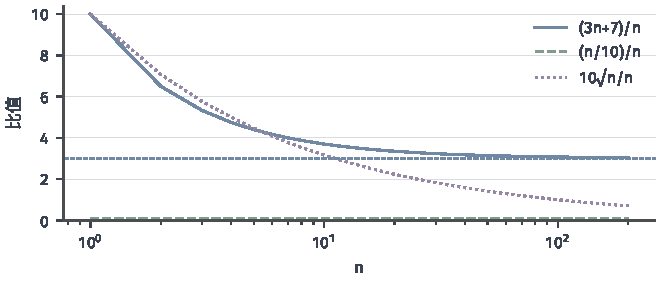
\includegraphics[width=112mm]{figures/01-mathematical-preliminaries-upper/00-shared/matplotlib/mathematical-language-combinatorics-analysis-optimization-comprehension-additions/asymptotic-ratios.pdf}
  \caption{三个解析数列除以$n$后的比值，展示整数$n=1,\ldots,200$，横轴为对数刻度。蓝、绿、紫线的极限分别为$3,0.1,0$。前两者对应$O(n)$而非$o(n)$，第三者对应$o(n)$；极限由正文中的表达式判断，有限范围曲线只帮助观察。}
  \label{fig:vol1-add-asymptotic-ratios}
\end{figure}

对最终为正的数列，若存在$c>0$使$a_n\geq cb_n$最终成立，记$a_n=\Omega(b_n)$；
同时满足$a_n=O(b_n)$与$a_n=\Omega(b_n)$，记$a_n=\Theta(b_n)$，表示同一数量级。
例如$3n+7=\Theta(n)$。这里的常数不随趋于无穷的$n$改变。
$n=O(n^2)$也成立，因此大$O$给出上界，不一定给出精确的增长阶。
这些记号在求导和局部近似中用来表达余项的大小。

\FloatBarrier

\section{实轴上的邻域与闭区间}
\label{sec:analysis-metric-measurement}
\label{sec:analysis-set-metric}

前几节的极限都在控制距离：$|a_n-a|<\varepsilon$说明第$n$项离极限不远，
$0<|x-a|<\delta$说明输入离中心不远。下一章研究一元函数的连续性、极值和积分时，还要反复回答三个问题：
“一个点附近”指哪些点；什么样的集合能留住其中点列的极限；
在闭区间每一点附近分别成立的控制，怎样合成对整个区间同时有效的控制。
本节依次用邻域与开闭集、闭集的序列判据和闭区间的有限子覆盖性质回答它们。

\subsection{开球、邻域与开闭集}

\paragraph{开球与邻域}
讨论一个点附近的变化，需要先指定哪些点算作离它足够近。

\begin{definition}[开球与邻域]
\label{def:analysis-open-ball}
设$x\in\mathbb R$，$r>0$。开区间
\[
 B(x,r)=\{y\in\mathbb R:|y-x|<r\}=(x-r,x+r)
\]
称为以$x$为中心、半径为$r$的\term{开球}（open ball）。若集合$V\subseteq\mathbb R$包含某个$B(x,r)$，就称$V$是$x$的邻域。
\end{definition}

在实轴上，开球就是以$x$为中心的对称开区间；用“球”这个名称，是为了后面换成平面或空间中的距离时沿用同一说法。
邻域只要求在$x$周围留出一段余量，本身不必是开区间。例如$[0,1]$是$1/2$的邻域，因为它包含$B(1/2,1/4)$；
它却不是端点$0$的邻域，因为每个$B(0,r)$都含有负数。

\paragraph{开集与闭集}
有了开球，就能检验一个集合是否在其中每个点周围都留有余量；对补集作同样检验，又得到闭集。

\begin{definition}[开集与闭集]
\label{def:analysis-open-closed-sets}
集合$U\subseteq\mathbb R$若对每个$x\in U$都存在$r>0$使$B(x,r)\subseteq U$，就称为\term{开集}（open set）；
集合$F\subseteq\mathbb R$若其补集$\mathbb R\setminus F$为开集，就称为\term{闭集}（closed set）。
\end{definition}

开区间$(a,b)$是开集：对其中的$x$，取$r=\min\{x-a,b-x\}$即可。
闭区间$[a,b]$是闭集，因为补集$(-\infty,a)\cup(b,\infty)$中每一点都能取到不碰到$[a,b]$的小球；
$[a,b]$本身不是开集，端点$a$周围的任何开球都含有区间外的点。
$\mathbb R$与空集既开又闭；但“不是开集”不等于“就是闭集”，例如$[0,1)$在$0$处不开，
它的补集在$1$处也不开，所以$[0,1)$两者都不是。
有限个开集的交仍是开集，可在各点取各个允许半径中最小的一个；无限多个开集的交未必开，
例如$\bigcap_{n\geq1}(-1/n,1/n)=\{0\}$。

\subsection{闭集的序列判据}

闭集由补集定义，使用时却常要问：一列点都在集合中，它的极限是否也在集合中？下面说明这两种说法等价。

\begin{lemma}[闭集的序列判据]
\label{lem:analysis-closed-sequence-criterion}
设$F\subseteq\mathbb R$。$F$是闭集，当且仅当：对每个取值于$F$的数列$(x_n)$，若$x_n\to x$，则$x\in F$。
\end{lemma}
\begin{proof}
若$F$闭而$x\notin F$，开集$\mathbb R\setminus F$包含某个$B(x,r)$。
收敛要求充分靠后的$x_n$落入这个开球，与$x_n\in F$矛盾。
反之，若$F$不闭，则补集不是开集，存在$x\notin F$，使每个$B(x,r)$都与$F$相交。
为每个$n$选$x_n\in F\cap B(x,1/n)$，便有$x_n\to x\notin F$，违反序列条件。
\end{proof}

例如$(0,1)$中的$1/n$趋于$0$，而$0\notin(0,1)$，所以$(0,1)$不是闭集。
闭与有界是不同的性质：$(0,1)$有界但不闭，$\mathbb R$闭但无界。
二者同时成立时，Bolzano--Weierstrass定理~\ref{thm:analysis-bounded-subsequence}给出收敛子列，
本引理又保证子列的极限仍在集合内；下一章的极值定理正是由此得到。

\subsection{闭区间的有限子覆盖性质}

\paragraph{开覆盖与有限子覆盖}

连续性在每一点给出一个邻域内的控制，但不同点的邻域大小可能不同。
要得到对整个闭区间同时有效的结论，需要从无限多个邻域中选出有限个，仍覆盖整个区间。
下面先规定“从一族开集中选出有限部分仍不遗漏”的含义。
\begin{definition}[开覆盖与紧致性]
\label{def:analysis-compactness}
设$K\subseteq\mathbb R$。一族开集的并包含$K$时，称它们为$K$的\term{开覆盖}（open cover）；
从中选出的有限个开集仍覆盖$K$时，称它们构成\term{有限子覆盖}（finite subcover）。
若$K$的每个开覆盖都存在有限子覆盖，则称$K$\term{紧致}（compact）。
\end{definition}
开覆盖本身可以有无限多个成员；有限子覆盖要求从原来的成员中挑选，而不是另换一组集合。

\paragraph{闭区间的紧致性}

闭区间里的点不会逃向无穷，收敛子列的极限也不会离开区间。
这两个条件使局部邻域覆盖不能一直要求加入新的成员。
\begin{theorem}[闭区间的有限子覆盖性质]
\label{thm:analysis-interval-finite-subcover}
实轴上的每个闭区间$[a,b]$都是紧致集。
\end{theorem}
\begin{proof}
$a=b$时选择一个包含该点的覆盖成员即可。设$a<b$，并给定$[a,b]$的开覆盖$\mathcal U$。
先证明这组覆盖有一个共同尺度：
\begin{equation}
 \exists r>0,\quad\forall x\in[a,b],\quad\exists U\in\mathcal U,
 \qquad B(x,r)\cap[a,b]\subseteq U.
\label{eq:analysis-cover-uniform-radius}
\end{equation}
若不存在这样的$r$，对每个$n$可选$x_n\in[a,b]$，使
$B(x_n,1/n)\cap[a,b]$不包含于任何一个覆盖成员。
有界数列$(x_n)$有子列$x_{n_k}\to x\in[a,b]$。
选$U\in\mathcal U$包含$x$，由开性取$\rho>0$使$B(x,\rho)\subseteq U$。
当$k$足够大时，$|x_{n_k}-x|<\rho/2$且$1/n_k<\rho/2$，
于是$B(x_{n_k},1/n_k)\subseteq B(x,\rho)\subseteq U$，产生矛盾。

有了共同半径$r$，把$[a,b]$分成有限个长度小于$r$的小区间。
每段任选一个点$x$，整段都落在$B(x,r)\cap[a,b]$内，故可由一个覆盖成员包含。
每段选择一个这样的成员，得到有限子覆盖。
\end{proof}

每个有界闭集$K\subseteq\mathbb R$也有此性质：先把它放入某个$[a,b]$，
再把$\mathbb R\setminus K$加入它的任意开覆盖，应用闭区间结论后删去这一补集。
有限子覆盖控制的是整个集合，而非只在几个已选点附近留出余量。图~\ref{fig:analysis-process-finite-open-cover}对照一个闭区间的有限覆盖与一个开区间上无法有限选取的覆盖族。
\begin{figure}[!htbp]
 \centering
 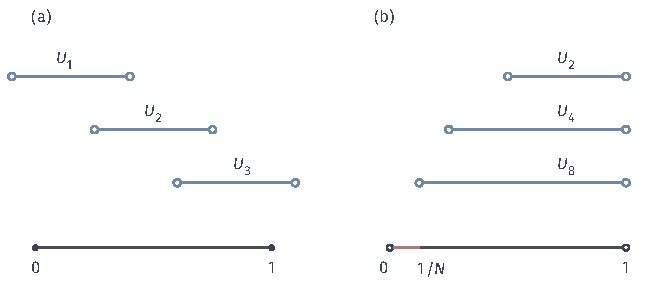
\includegraphics[width=112mm]{figures/01-mathematical-preliminaries-upper/01-mathematical-language-combinatorics-analysis-optimization/tikz/chapter3-concept-processes/finite-open-cover.pdf}
 \caption{(a) 三个开区间$(-0.1,0.4)$、$(0.25,0.75)$、$(0.6,1.1)$覆盖$[0,1]$。(b) $U_n=(1/n,1)$（$n\geq2$）覆盖$(0,1)$；只选有限多个时，设最大下标为$N$，红段$(0,1/N]$仍未覆盖。图只画$U_2,U_4,U_8$；右侧的失败由最大下标论证，不是有限图像的猜测。}
 \label{fig:analysis-process-finite-open-cover}
\end{figure}

以上定义只用到实数之间的距离$|x-y|$。把它换成欧氏距离$\lVert\bm x-\bm y\rVert_2$，
就得到$\mathbb R^d$中的开球$B(\bm x,r)=\{\bm y:\lVert\bm y-\bm x\rVert_2<r\}$、邻域、开集与闭集，
闭集的序列判据连同证明逐字成立；线性空间部分与多元微积分章使用的正是这些欧氏版本。
欧氏空间中闭有界集的子列性质在多元微积分章逐坐标证明，一般距离下的开闭集与紧致性在第~\ref{chap:metric-spaces}章讨论。

\FloatBarrier


\FloatBarrier
\section{本章小结}
\label{sec:function-limits-summary}

$|\rho|<1$时等比序列趋于零，有限几何和趋于$1/(1-\rho)$。
极限先规定趋近的含义，再分别研究怎样计算极限、怎样保证极限存在；后者依赖实数的确界原理。
级数把累计过程写成部分和的极限；重排改变项的顺序，分组保留次序而合并相邻项，二者的结论不能混用。
实轴上的开球与邻域规定局部范围，开闭集和闭集的序列判据描述极限的归属。
闭区间的紧致性使局部控制能够合成整体控制，后续微积分将据此研究连续性、变化与累计；
一般度量规则与完备性在“度量空间”章统一讨论。
